% !TeX root = ../main.tex
\addcontentsline{toc}{section}{Introduction}
\section*{Introduction}
Les chapitres précédents ont exposé la stratégie de migration et sa réalisation script par script. Le présent chapitre adopte un angle différent : il décrit la chaîne outillée qui a
rendu possible cette réalisation, depuis la connexion sécurisée à l'infrastructure de l'opérateur telecom
jusqu'à la visualisation des résultats dans l'IHM Ni2. Maîtriser cette chaîne, c'est garantir la
reproductibilité, la traçabilité et la sécurité de chaque opération réalisée en contexte de production.

\section{Environnement de Travail}
L'environnement de travail repose sur un ensemble d'outils spécialisés, chacun couvrant une
responsabilité précise dans la chaîne de valeur du projet. Leur articulation forme un écosystème
cohérent allant de l'accès sécurisé aux bases de données jusqu'au versioning du code de migration.

\subsection{Accès sécurisé — Cisco VPN Client}
L'ensemble des ressources du projet est hébergé dans
l'infrastructure réseau d'Inetum / opérateur telecom, accessible uniquement via un tunnel VPN sécurisé.
Le client Cisco VPN (version 5.0.07.0440) est utilisé pour établir cette connexion IPSec/UDP vers le
concentrateur 196.201.192.2 (entrée CF)

\begin{figure}[H]
    \centering 
    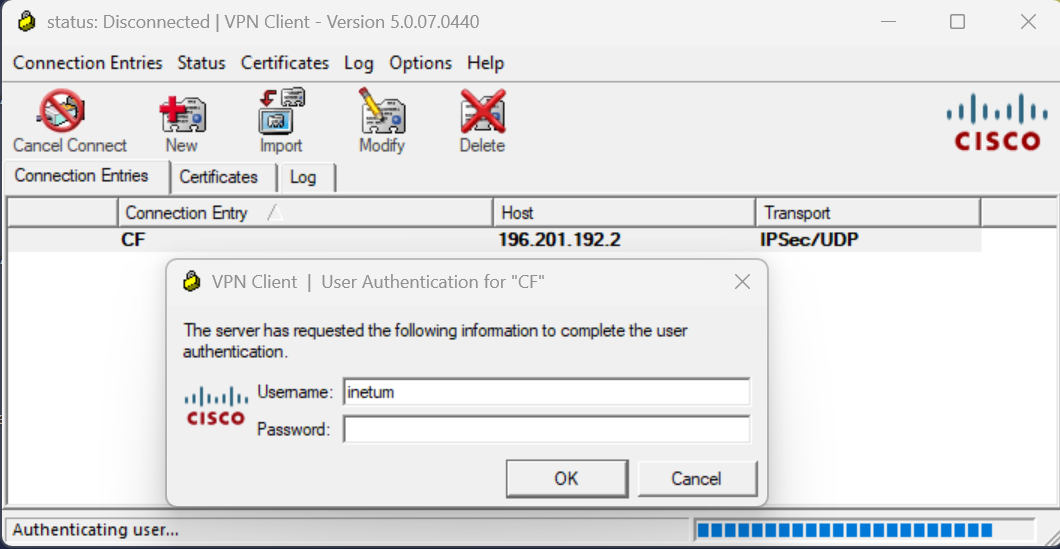
\includegraphics[width=0.8\textwidth]{images/chapitre 4/vpn.png}
    \caption{Authentification VPN Cisco}    
\end{figure}

\begin{itemize}
    \item Protocole : IPSec/UDP — garantit le chiffrement de bout en bout de tout flux de données (scripts SQL, CSV, commandes Shell).
    \item Compte d'accès dédié projet (inetum) avec authentification par identifiant + mot de passe géré par l'équipe sécurité Inetum.
    \item La connexion VPN est le pré-requis absolu de toute session de travail : aucun outil de la chaîne ne fonctionne sans elle.
\end{itemize}

\subsection{Accès aux bases de données — DBeaver}

\begin{tabular}{cl}
    
\includegraphics[height=2em]{images/chapitre 4/dbeaver.jpg} & \begin{minipage}[c]{0.85\textwidth} \textbf{DBeaver} est l'environnement central d'exploration et de développement SQL. Il offre une vue unifiée sur les deux bases sources du projet, permettant de naviguer dans les schémas, d'exécuter des requêtes et d'exporter les résultats en CSV directement exploitables par le pipeline Ni2. \end{minipage} \\[1em]
\end{tabular}

\begin{itemize}
    \item Connexion Oracle GAIA — driver JDBC Oracle, accès en lecture seule au schéma d'inventaire réseau.
    \item Connexion MSSQL CRM — driver JDBC SQL Server, accès aux 900+ tables pour la rétro-ingénierie et les scripts SQL du Jalon 4.
    \item Fonctionnalité clé : l'explorateur de schéma (ER Diagram) a permis de visualiser les relations entre tables CRM lors de la phase de rétro-ingénierie.
\end{itemize} 

\begin{figure}[H]
    \centering
    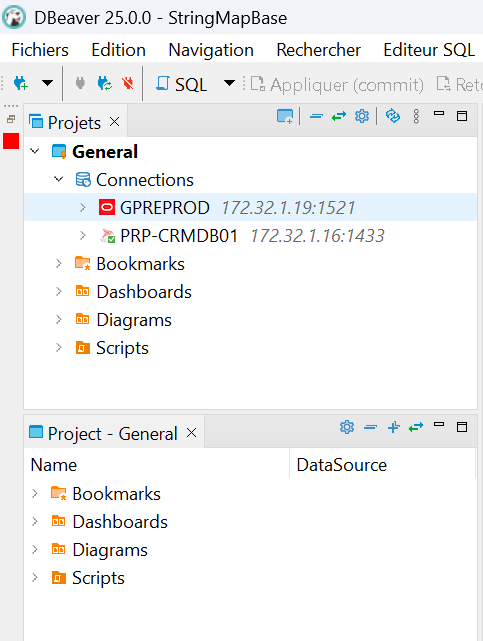
\includegraphics[width=0.8\textwidth]{images/chapitre 4/cnxDbeaver.png}
    \caption{DBeaver : double connexion GAIA et CRM }
\end{figure}

\subsection{Pilotage du serveur distant — MobaXterm}
\begin{tabular}{cl}
    
\includegraphics[height=2em]{images/chapitre 4/mobaxterm.jpg} & \begin{minipage}[c]{0.85\textwidth} \textbf{Mobaxterm } est le point d'entrée unique pour toutes les opérations sur le serveur Ni2 distant. Il
combine terminal SSH, transfert de fichiers SFTP et tunneling X11 dans une interface unifiée, ce qui
simplifie considérablement le workflow de déploiement. \end{minipage} \\[1em]
\end{tabular}
\begin{itemize}
    \item Connexion SSH au serveur DEV Ni2 après établissement du tunnel VPN.
    \item Transfert des fichiers de configuration (.cred, CSV pivots) via SFTP intégré.
    \item Exécution du build de l'application Ni2 et déploiement des Custom Fields avant chaque import.
    \item Redémarrage contrôlé des services Ni2 pour prise en charge des nouveaux champs personnalisés déployés
\end{itemize}

\begin{figure}[H]
    \centering
    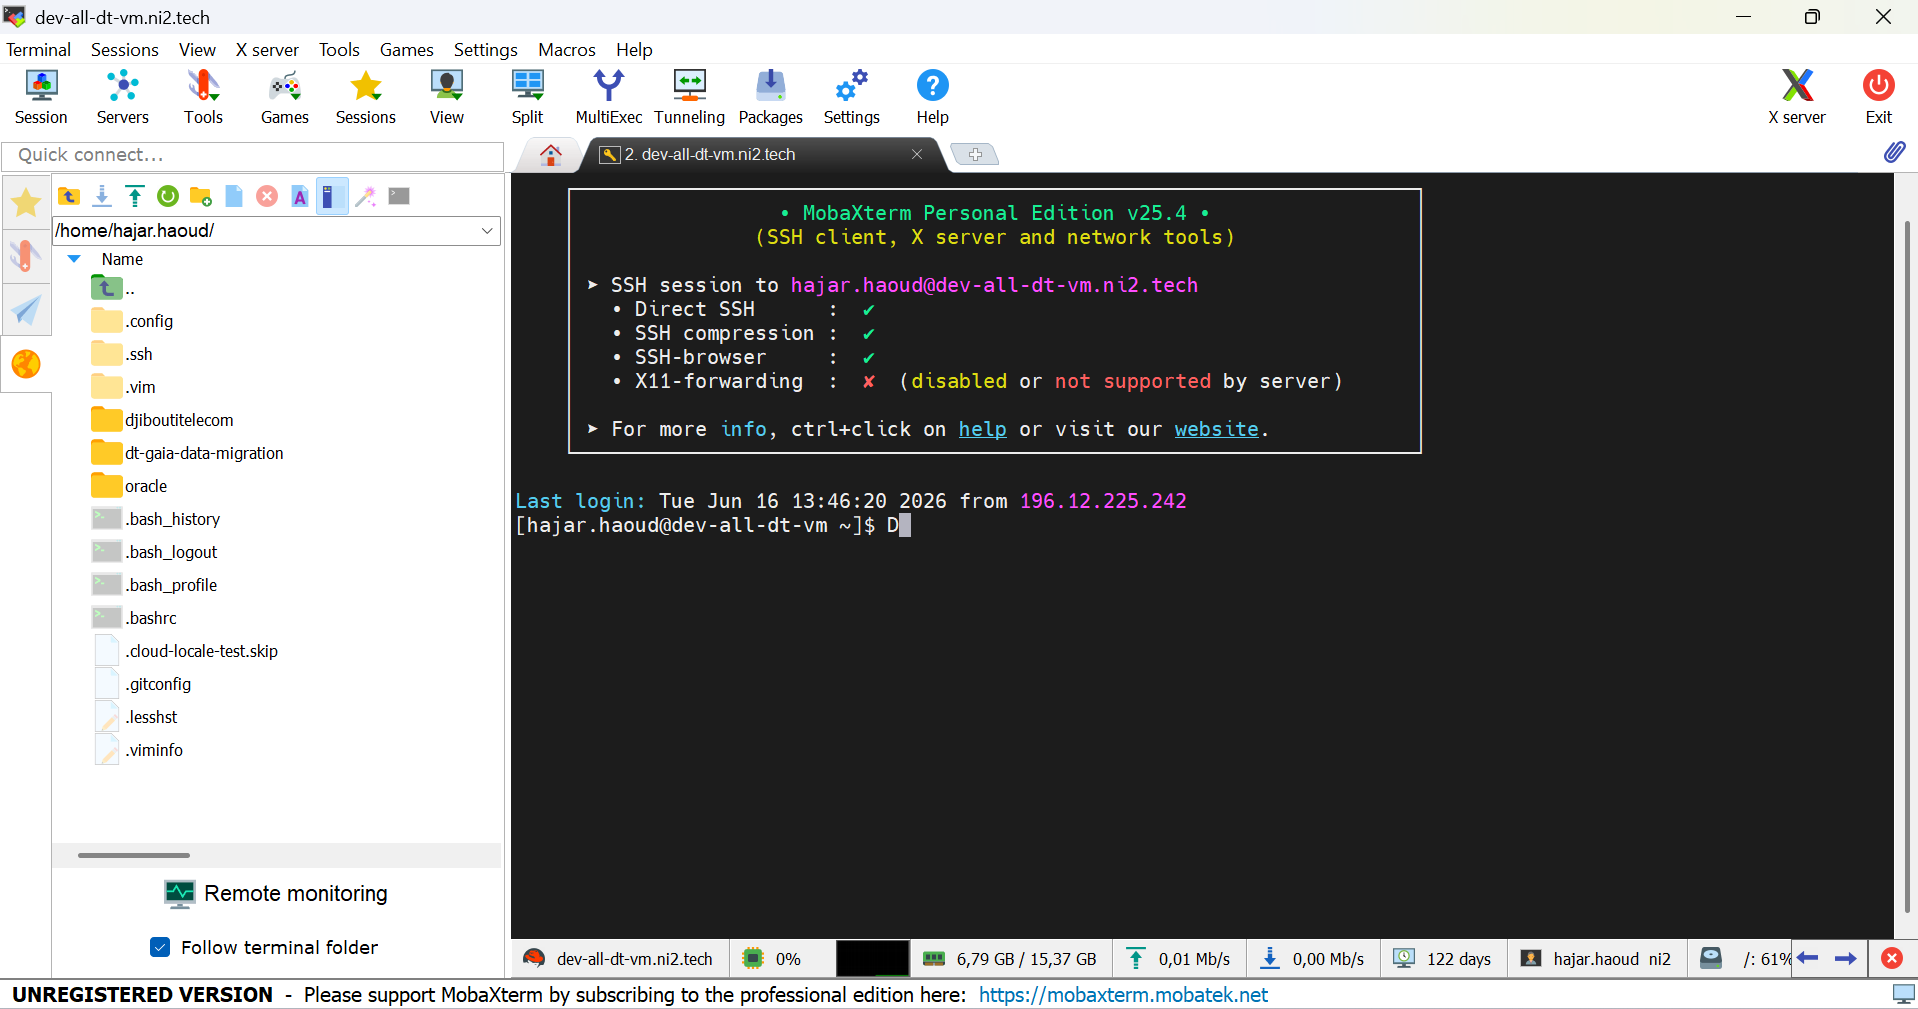
\includegraphics[width=0.8\textwidth]{images/chapitre 4/sessionmobaxterm.png}
    \caption{ MobaXterm : session SSH active sur le serveur DEV Ni2}
\end{figure}

\subsection{Développement des scripts — Visual Studio Code}
\begin{tabular}{cl}
    
\includegraphics[height=2em]{images/chapitre 4/vslogo.jpg} & \begin{minipage}[c]{0.85\textwidth} \textbf{VS Code } est l'environnement de développement principal pour l'écriture et la maintenance de l'ensemble des scripts du projet. Son extensibilité (extensions SQL, Java, GitLens) et son intégration Git native en font un outil central de la chaîne de production. \end{minipage} \\[1em]
\end{tabular}

\begin{itemize}
    \item Scripts SQL (CRM Jalon L4) avec coloration syntaxique et autocomplétion.
    \item Scripts Shell (./ni2SyncMSSQL.sh) pour l'orchestration des imports.
    \item Gestion des branches Git et visualisation des diffs avant chaque push sur le dépôt dt-gaia-data-migration.
\end{itemize}

\begin{figure}[H]
    \centering
    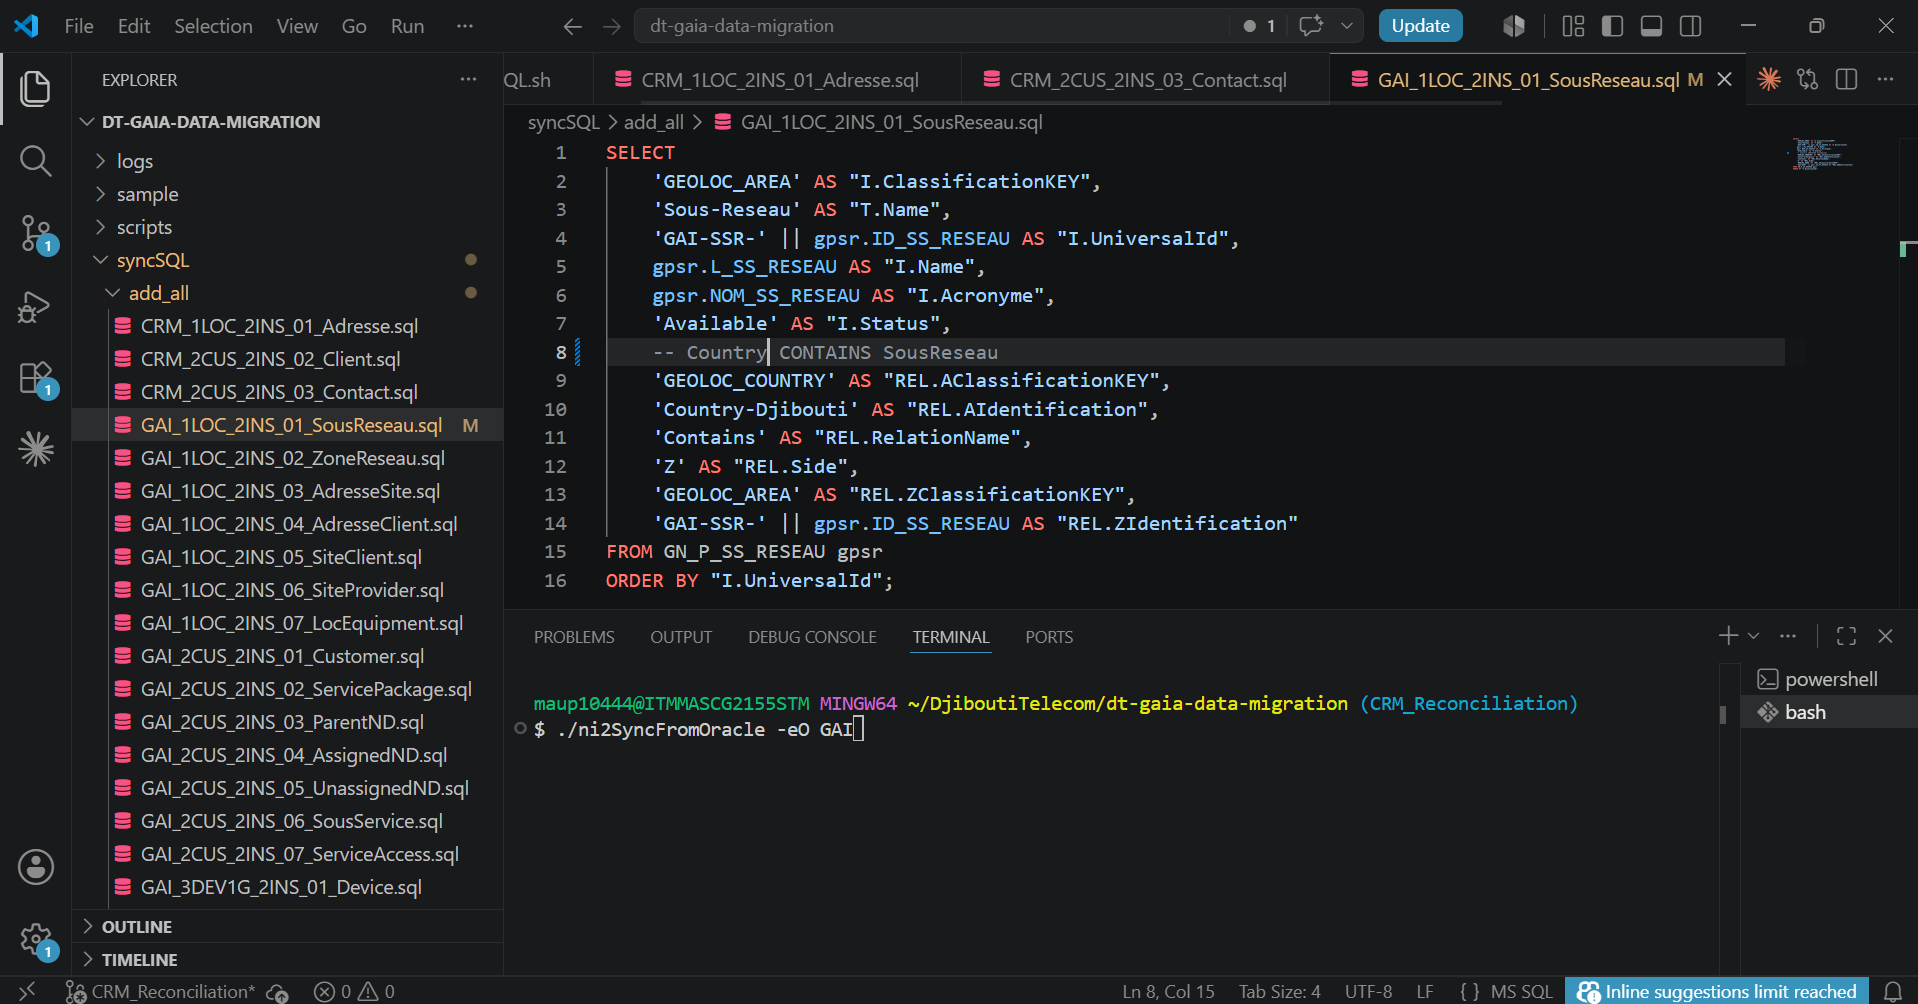
\includegraphics[width=0.8\textwidth]{images/chapitre 4/vs.png}
    \caption{ VS Code : développement des scripts SQL et Shell}
\end{figure}

\subsection{Versioning et collaboration — Git \& Bitbucket}
Tout le code produit (scripts SQL, fichiers de mapping, configurations Ni2) est versionné sur deux
dépôts Bitbucket dédiés au projet de l'opérateur telecom. Le versioning garantit la traçabilité complète des
modifications et permet le rollback à tout état antérieur en cas d'erreur.

\begin{itemize}
    \item \textbf{dt-gaia-data-migration :} dépôt principal des scripts de migration GAIA et CRM, organisé par thème (locations, customers, devices, crm).
    \item \textbf{Deuxième dépôt : }configurations Ni2, Custom Fields, fichiers customisations et scripts de déploiement.
    \item Workflow de branches : HAH_1LOC (branche) → Pull Request → revue → merge sur main après validation en DEV.
\end{itemize}

\begin{figure}[H]
    \centering
    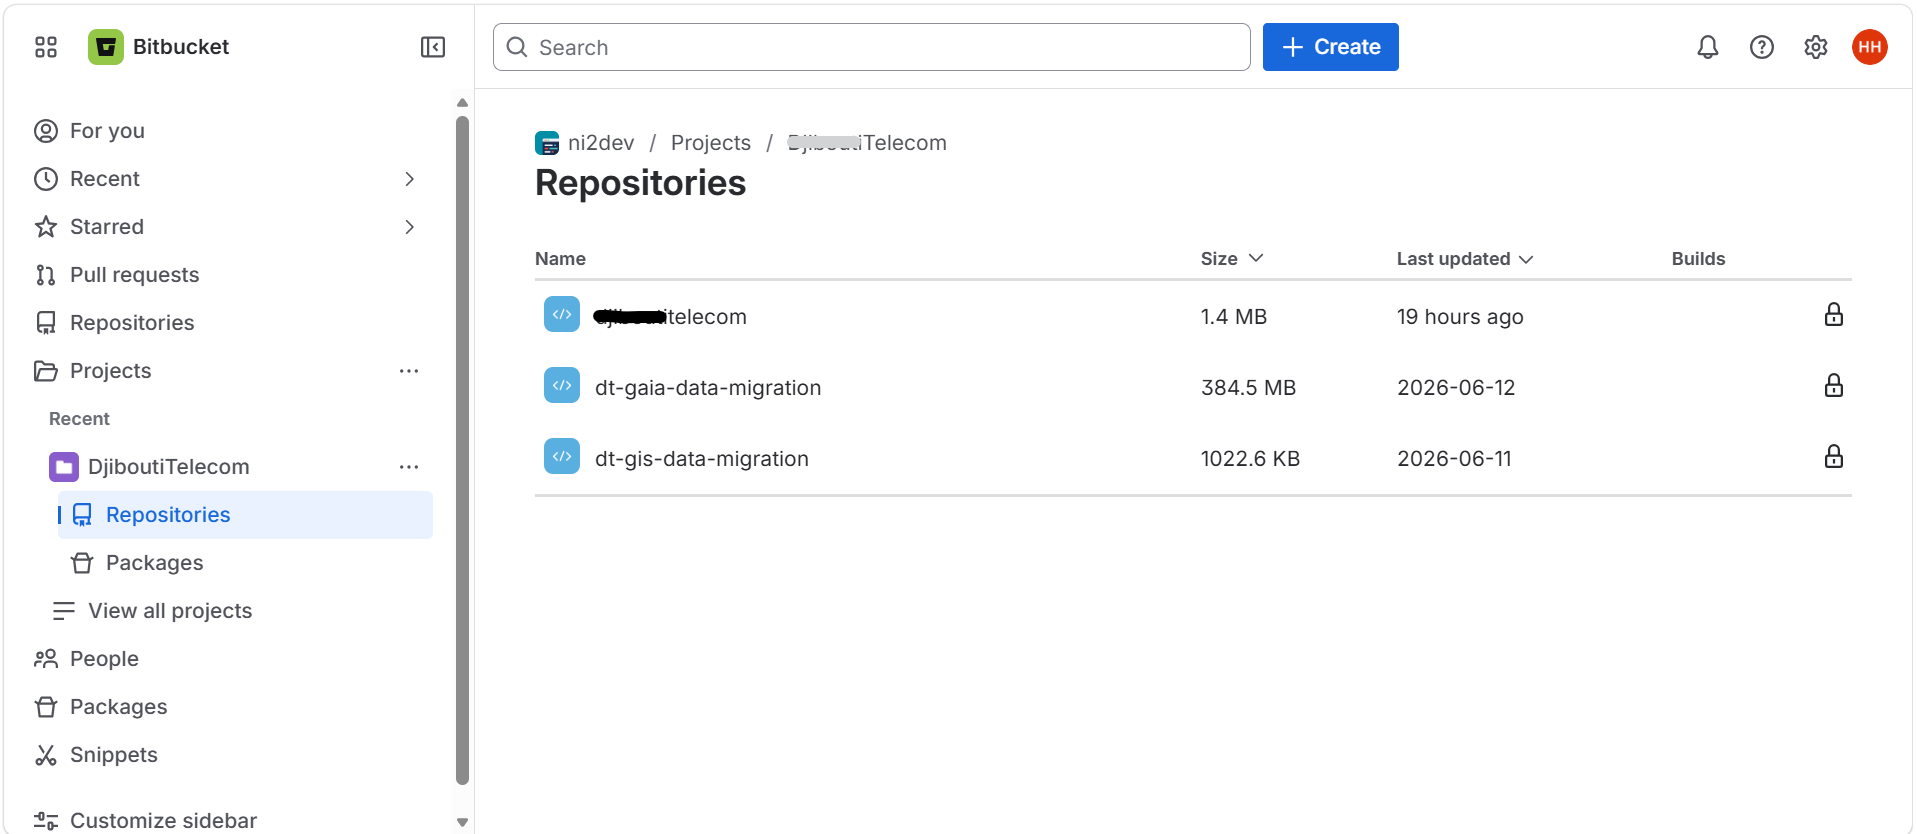
\includegraphics[width=0.8\textwidth]{images/chapitre 4/bitbucket.png}
    \caption{ Bitbucket : dépôt dt-gaia-data-migration et ***telecom}
\end{figure}

\subsection{Documentation et modélisation — Excel \& Draw.io}    
\begin{tabular}{cl}
    
\includegraphics[height=2em]{images/chapitre 4/excel.jpg} & \begin{minipage}[c]{0.85\textwidth} \textbf{Excel }est l'outil de documentation structurée du projet. Le fichier de mapping CRM/GAIA → Ni2, le Dossier de Test de Recette (DTR) et les tableaux de bord de suivi des KPIs de migration sont tous maintenus dans des classeurs Excel partagés sur le dépôt Bitbucket.   \end{minipage} \\[4em]
    
\includegraphics[height=2em]{images/chapitre 4/draw.io.png} & \begin{minipage}[c]{0.85\textwidth} \textbf{Draw.io }est utilisé pour la modélisation des données et des flux de processus. Les diagrammes d'inventaire Ni2, les schémas ETL et les modèles de données des thèmes GAIA/CRM ont été produits avec cet outil et intégrés dans les livrables projet. \end{minipage}
\end{tabular}

\subsection{Vue d'ensemble — Articulation des outils}
Le tableau suivant récapitule les outils utilisés tout au long du projet, leur rôle spécifique ainsi que leur fréquence d'utilisation dans le workflow de migration :
\begin{table}[H]
    \centering
    \renewcommand{\arraystretch}{1.6}
    \resizebox{\textwidth}{!}{ % Pour s'assurer que le tableau tient sur la largeur de la page
    \begin{tabular}{|l|p{6.5cm}|p{6.5cm}|}
        \hline
        \rowcolor{iNavy} 
        \textbf{\color{white} Outil} & \textbf{\color{white} Rôle dans le projet} & \textbf{\color{white} Moment d'utilisation} \\ \hline
        
        \textbf{Cisco VPN} & Accès sécurisé à l'infrastructure réseau de l'opérateur. & Systématique --- préalable à toute session de travail. \\ \hline
        
        \textbf{DBeaver} & Exploration et requêtage SQL (Oracle + MSSQL). & Analyse GAIA, rétro-ingénierie CRM, validation des extractions. \\ \hline
        
        \textbf{MobaXterm} & Terminal SSH + transfert de fichiers (SFTP). & Déploiement \textit{Custom Fields}, build Ni2, redémarrage des services, import de données. \\ \hline
        
        \textbf{VS Code} & Écriture et maintenance des scripts. & Développement des scripts SQL, Shell et Python. \\ \hline
        
        \textbf{Git / Bitbucket} & Versionnage et collaboration. & Continu --- \textit{commit} après chaque thème validé. \\ \hline
        
        \textbf{Excel} & Mapping et documentation. & Conception du mapping, rédaction du DTR, suivi des KPIs de migration. \\ \hline
        
        \textbf{Draw.io} & Modélisation et diagrammes. & Conception des modèles de données et des diagrammes de flux. \\ \hline
    \end{tabular}
    }
    \caption{Stack technologique et outils de travail}
    \label{tab:stack_outils}
\end{table}

\section{ Processus de Déploiement — Du Script à la Production}
Chaque livraison de scripts vers l'environnement DEV Ni2 suit un workflow en six étapes ordonnées.
Ce processus garantit que rien n'est déployé sans avoir été versionné, et qu'aucun import n'est lancé
sur un environnement dont les pré-requis ne sont pas vérifiés.


\begin{figure}[H]
    \centering
    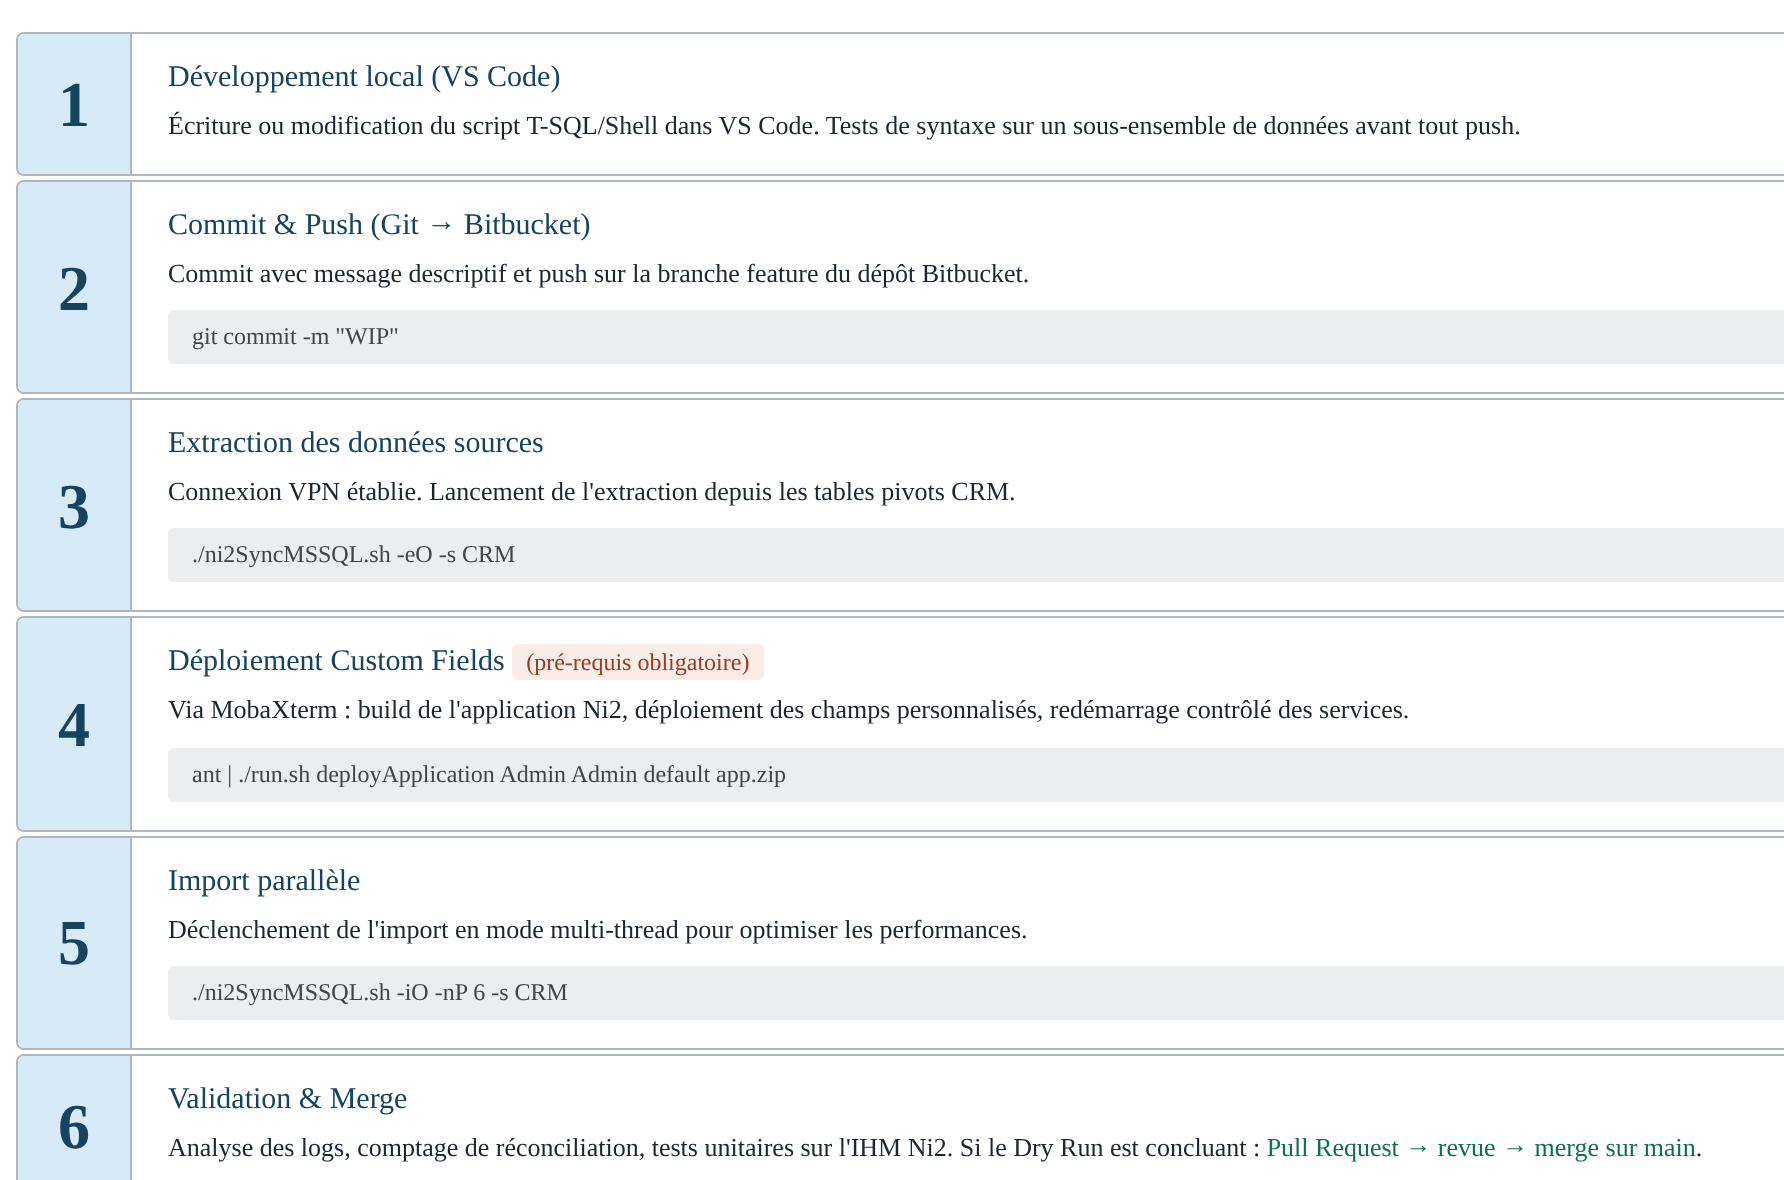
\includegraphics[width=0.8\textwidth]{images/chapitre 4/flux.png}
    \caption{Pipeline de déploiement en 6 étapes}
\end{figure}

\monBloc{\textbf{Note :} La séparation stricte entre les étapes 3 (extraction) et 4 (déploiement Custom Fields) est une leçon apprise en cours de projet : lancer l'import avant le redémarrage des services Ni2 produit des erreurs silencieuses difficiles à diagnostiquer. La checklist de déploiement formalise cette séquence pour tous les membres de l'équipe}

\textbf{Schéma du workflow Git}
\begin{figure}[H]
    \centering
    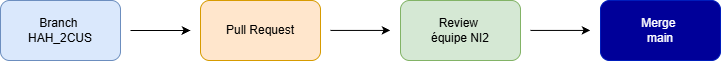
\includegraphics[width=0.8\textwidth]{images/chapitre 4/workflow git .drawio.png}
    \caption{Workflow Git du projet : de la branche créée au merge sur main}    
\end{figure}

\section{Visualisation Interface Ni2}
L'interface Ni2 (Unified Inventory) \textit{(https://dev-dt.ni2.tech)} est le tableau de bord final où se matérialisent tous les efforts de migration. Chaque objet importé, chaque relation établie, chaque attribut calculé sont consultables et navigables dans cette IHM web. Les six captures ci-dessous illustrent le parcours complet de validation d'un client importé : depuis la navigation dans le menu jusqu'à la vue schématique de ses relations.

\subsection{Tableau de bord Ni2 DEV — Navigation et accès}
L'accès à l'environnement DEV Ni2 (compte HHaoud) ouvre le tableau de bord principal. Le menu latéral expose les modules disponibles selon les habilitations définies dans le LLD : Administration, Gestion des commandes (Clients, Commandes de services), Emplacement, Centre de services, etc. La séquence \textbf{Gestion des commandes -> Clients -> Rechercher} est le point d'entrée pour valider les données migrées depuis le CRM.

\begin{figure}[H]
    \centering
    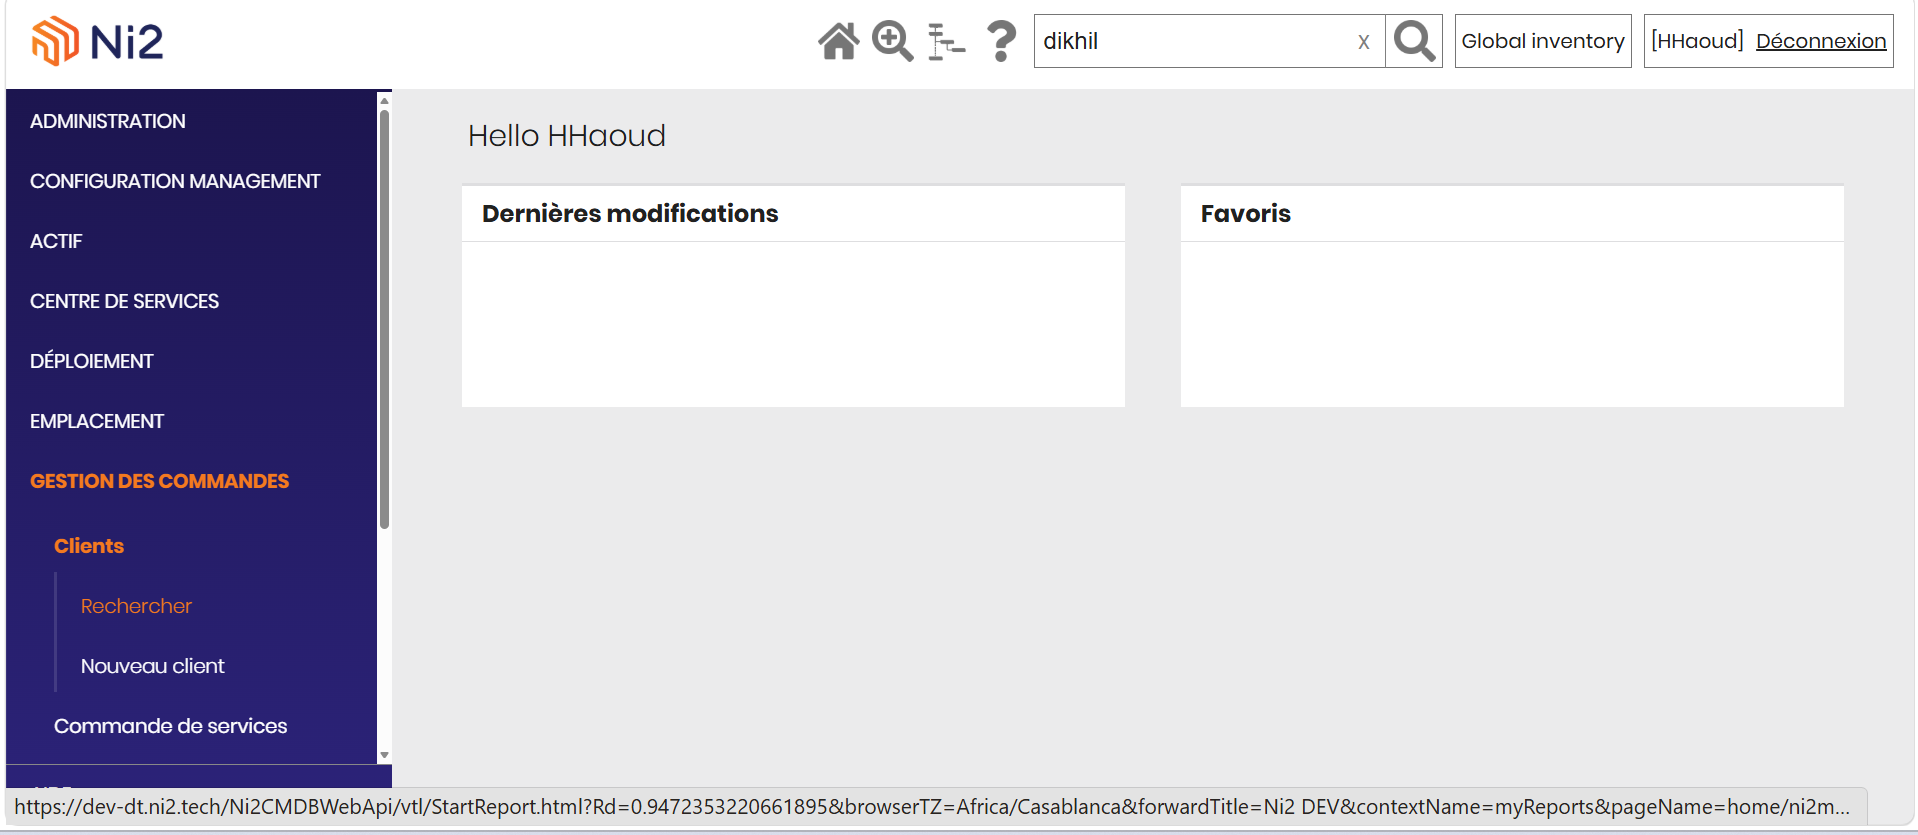
\includegraphics[width=0.8\textwidth]{images/chapitre 4/tableaubord.png}
    \caption{Tableau de bord Ni2 DEV (HHaoud) — menu Gestion des commandes actif}
\end{figure}

\subsection{Recherche clients — Volumétrie post-migration}
La recherche sans filtre retourne 27 127 items, confirmant que l'injection massive de données depuis GAIA s'est correctement effectuée. Ce chiffre constitue le premier KPI de validation de volume : l'ensemble des clients actifs du système source est présent et accessible dans Ni2. La popup de recherche offre un filtrage multi-critères (identifiant, nom, type, numéro client, statut) permettant de cibler rapidement un cas de test.

\begin{figure}[H]
    \centering
    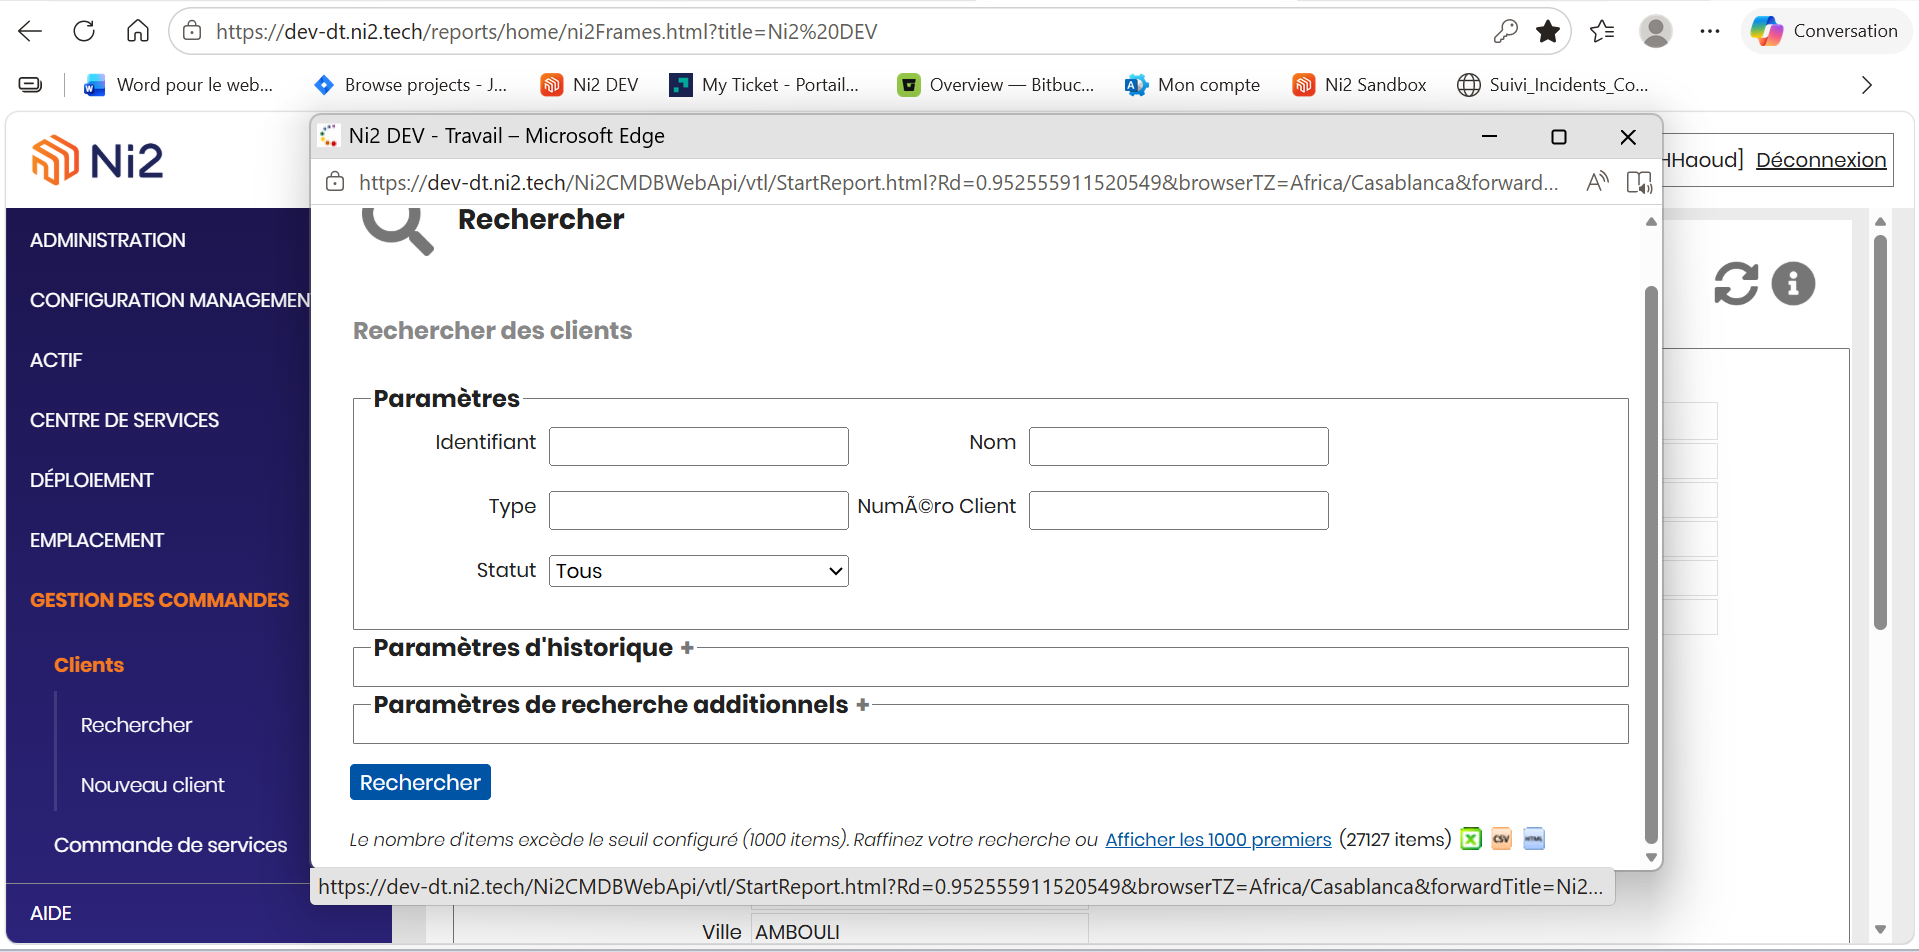
\includegraphics[width=0.8\textwidth]{images/chapitre 4/recherche.png}
    \caption{Module Recherche clients Ni2 : 27 127 clients importés détectés (KPI de volume)}
\end{figure}

\subsection{Fiche client importée — Test unitaire }
Le client ETS ABDALLAH ABDOULATIF (ID Ni2 : ACT-01652951, numéro client CRM : 9631) est sélectionné comme cas de test représentatif. Sa fiche affiche les attributs attendus après migration : type Generic Customer, statut Actif, et l'adresse complète : 27, Rue DE SOLEILLET, Q.COMMERCIAL, ***-VILLE. L'adresse est cliquable et pointe vers l'objet Adresse Ni2 correspondant (ADD-03163584), validant la relation \textbf{Consumes}.

\begin{figure}[H]
    \centering
    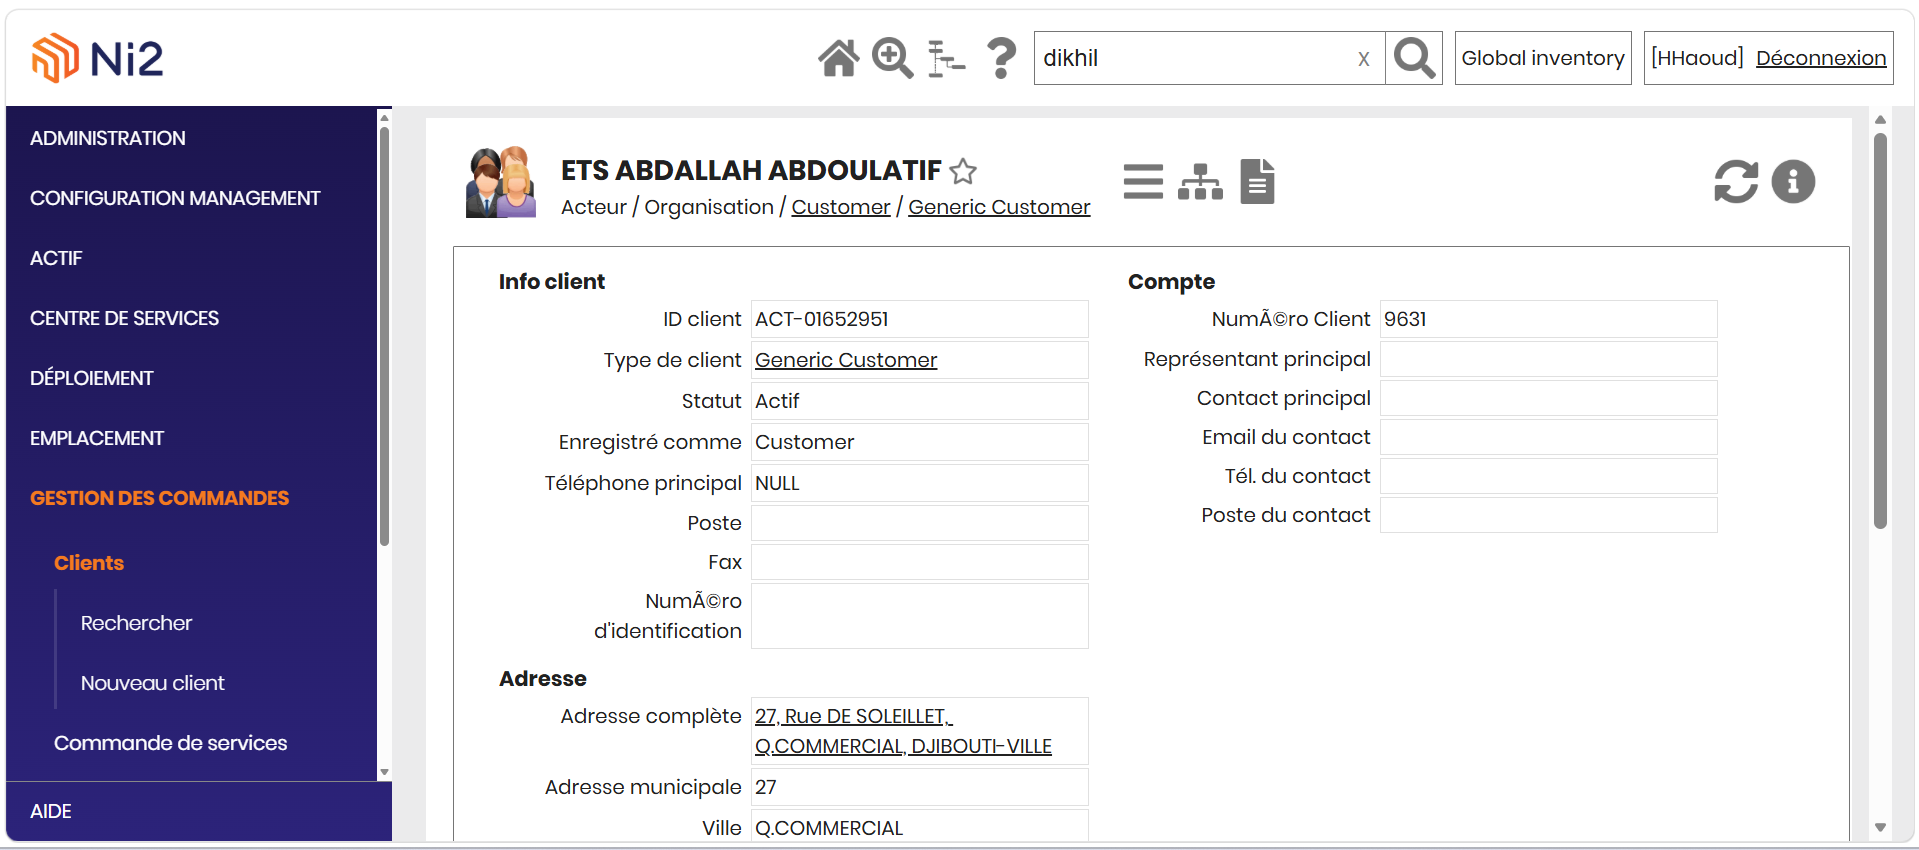
\includegraphics[width=0.8\textwidth]{images/chapitre 4/client.png}
    \caption{Fiche client}
\end{figure}

\subsection{Panneau Propriétés — Universal Id et champs CRM}
Le panneau \textbf{Propriétés} expose les attributs techniques du client. L'ID universel Org0002758 est la clé de réconciliation entre le CRM et GAIA, c'est via cet identifiant que le système garantit l'unicité du client dans Ni2 (zéro doublon). Les champs Catégorie = Professionnel et Document d'identification
= Initialisation sont alimentés directement depuis les colonnes discriminantes du GAIA, conformément au fichier de mapping Excel.

\begin{figure}[H]
    \centering
    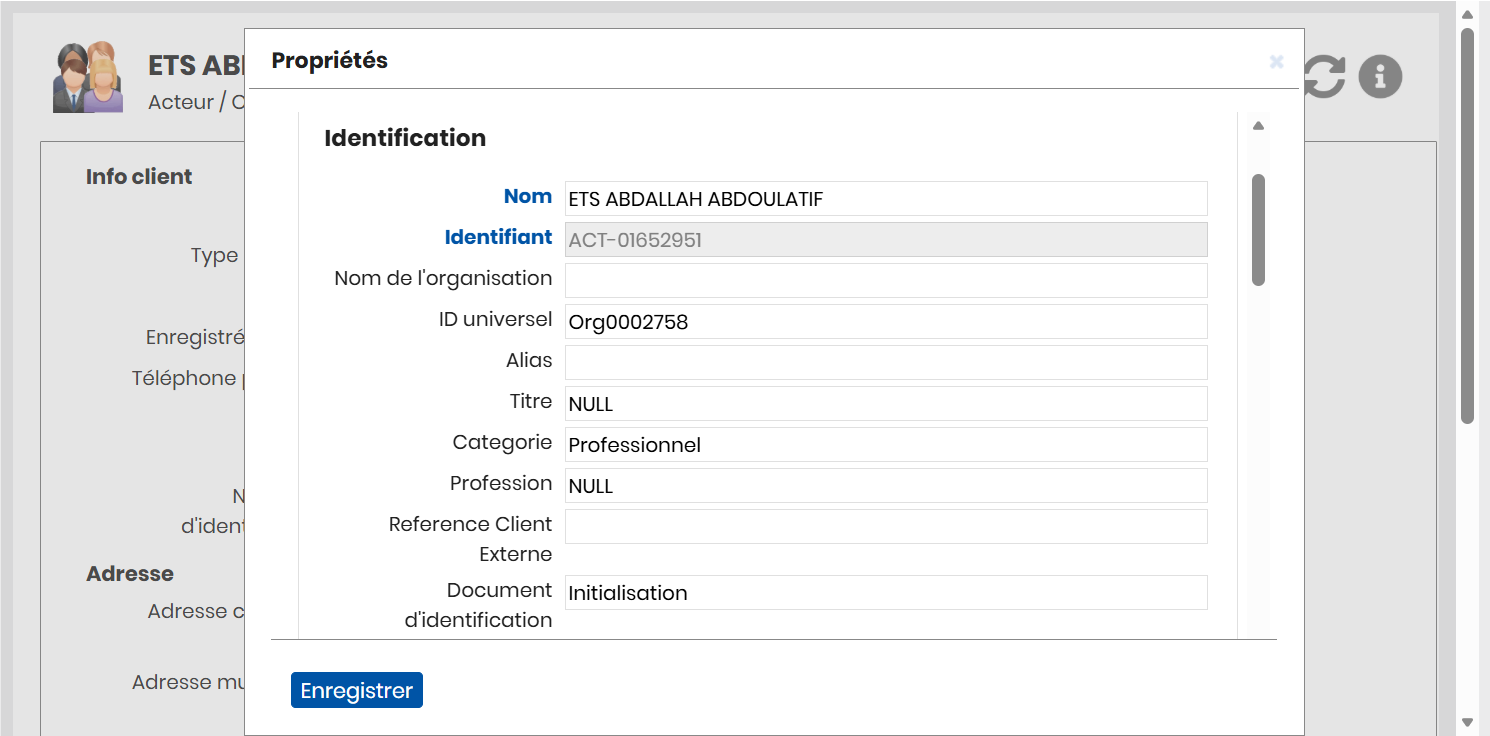
\includegraphics[width=0.8\textwidth]{images/chapitre 4/fiche.png}
    \caption{fiche de propriétés}
\end{figure}

\subsection{Onglet Dépendances — Relations importées}
L'onglet Dépendances révèle les deux relations établies automatiquement par les scripts d'import :
\begin{itemize}
    \item \textbf{ResponsibleFor(Customer) } -> Operateur telecom (ACT-00000002, ID Universel MSP-DT) : relation rattachant le client à l'opérateur en tant que Main Service Provider, créée automatiquement lors de l'import Actor.
    \item \textbf{Consumes(Main) } -> Adresse ADD-03163584 (27, Rue DE SOLEILLET, Q.COMMERCIAL, ***-VILLE, ID Universel ADR-Org0002758) : relation construite via la table Client du script SQL Customer.
\end{itemize}
Ces deux relations confirment que la migration ne s'est pas limitée à importer des objets isolés mais a reconstruit l'intégralité du graphe de dépendances défini dans le LLD fonctionnel.

\begin{figure}[H]
    \centering
    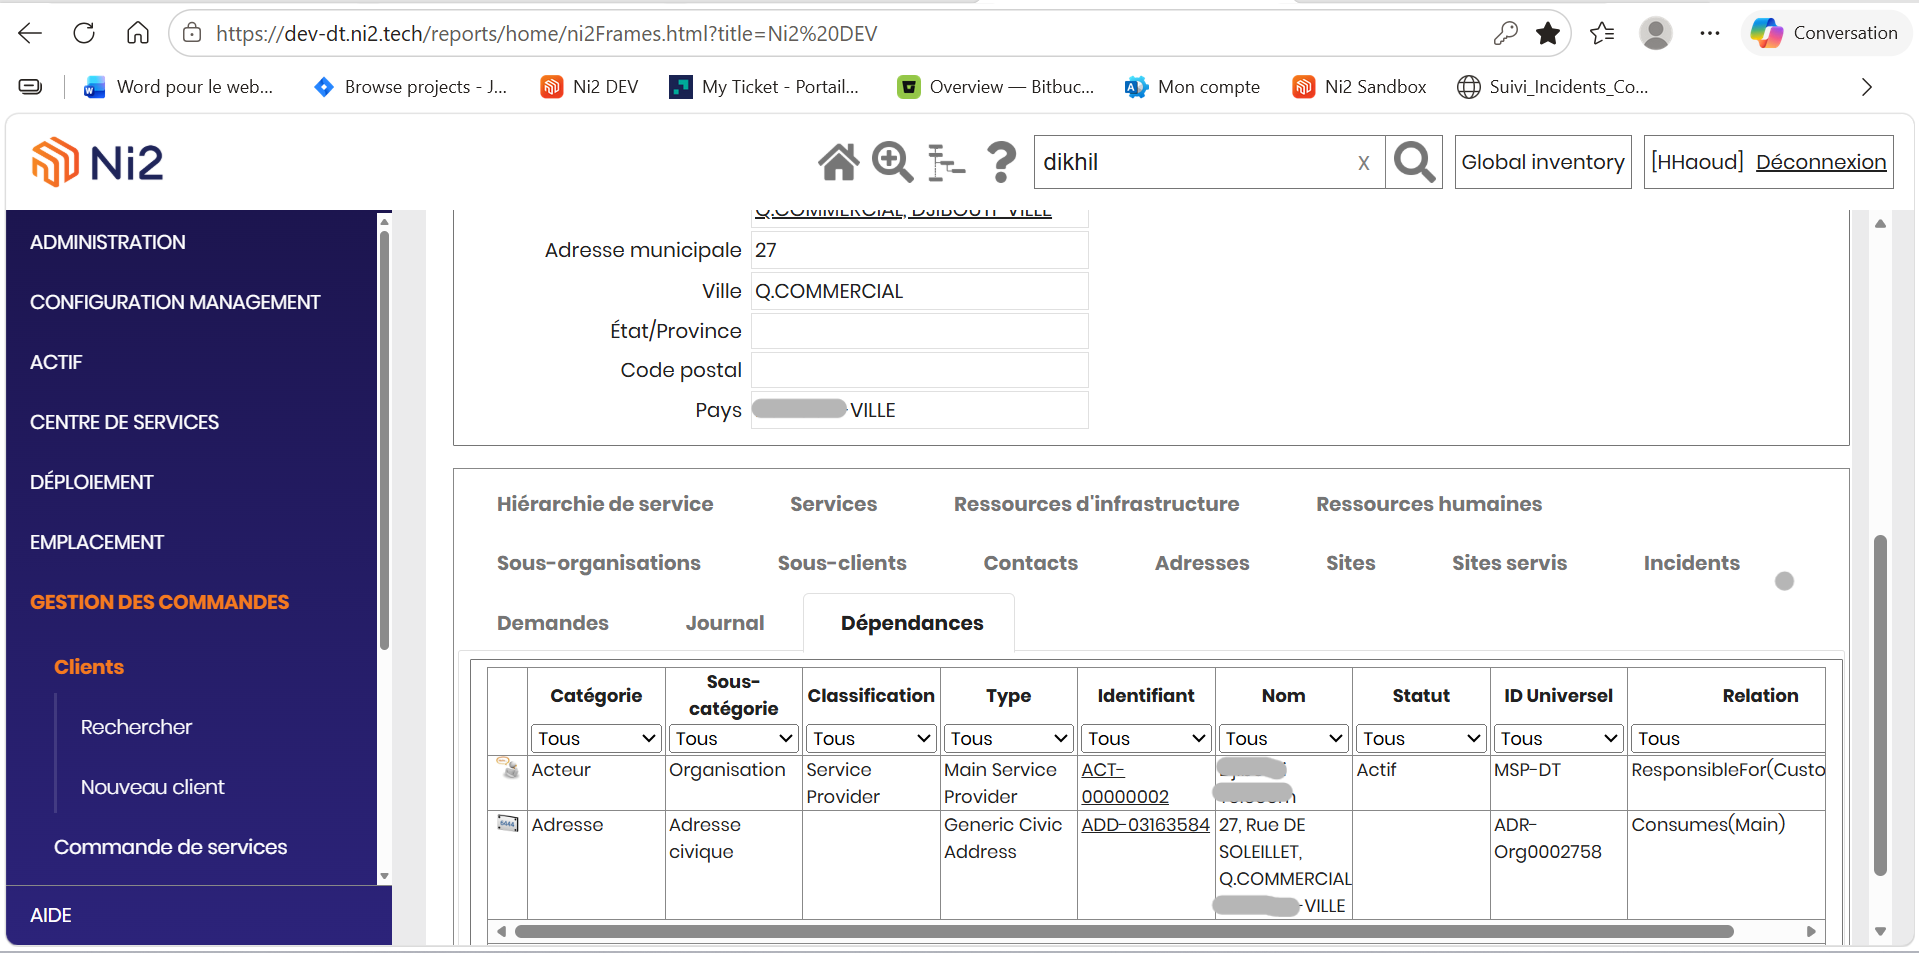
\includegraphics[width=0.8\textwidth]{images/chapitre 4/dependance.png}
    \caption{Onglet Dépendances }
\end{figure}

\subsection{Vue Schématique — Graphe relationnel}
La Schematic View Ni2 matérialise graphiquement le résultat de la migration : le client ETS ABDALLAH ABDOULATIF apparaît comme nœud central, relié à son adresse via Consumes(Main) et à Opérateur Telecom via ResponsibleFor(Customer). Ce graphe est la preuve visuelle la plus
parlante de la réussite de chaque jalon  : la structure relationnelle définie dans le modèle de données Ni2 est effectivement instanciée dans la base, sur des données réelles issues du CRM.

\begin{figure}[H]
    \centering
    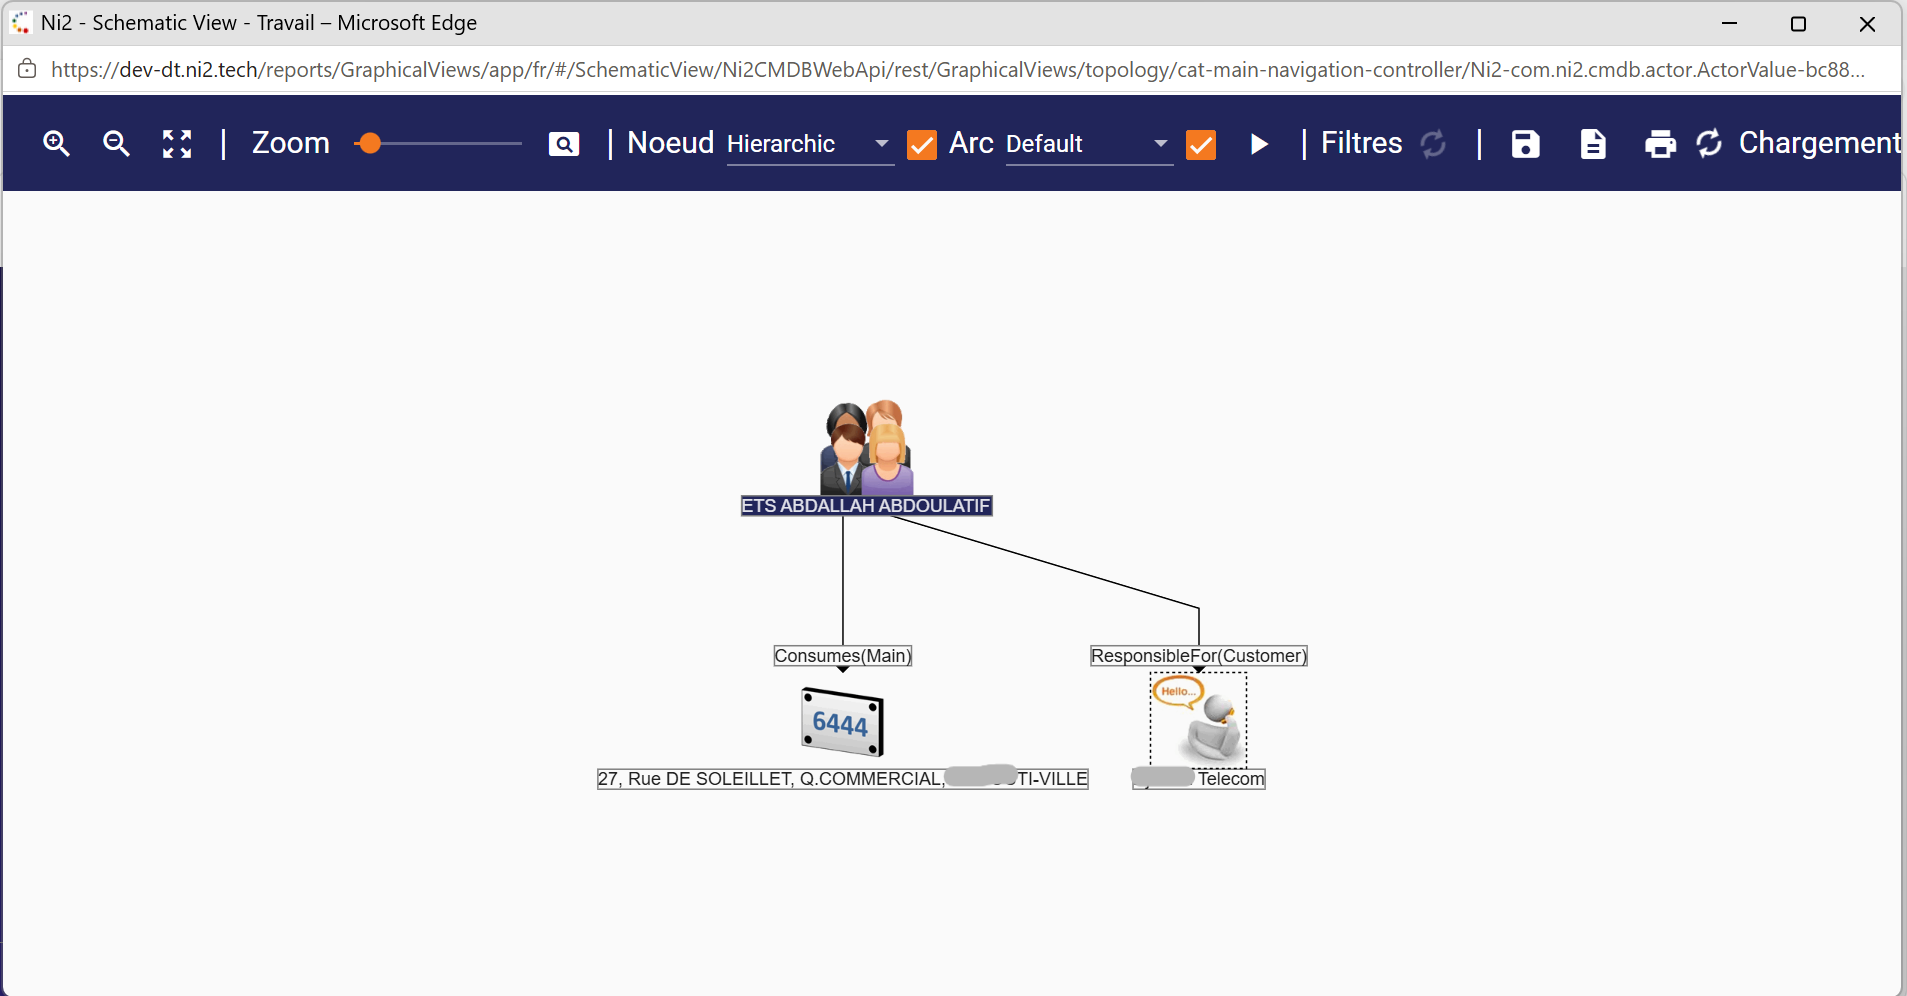
\includegraphics[width=0.8\textwidth]{images/chapitre 4/vueSchematique.png}
    \caption{Vue Schématique}
\end{figure}



\newpage
\addcontentsline{toc}{section}{Conclusion}
\section*{Conclusion}
Ce chapitre a mis en lumière la dimension technique transversale du projet : la chaîne outillée qui articule sept outils complémentaires pour former un environnement de production cohérent, sécurisé et traçable.\\

Le Cisco VPN sécurise chaque session par un tunnel IPSec/UDP. DBeaver offre une fenêtre unifiée sur les deux bases sources, Oracle GAIA et MSSQL CRM, rendant possible l'exploration et le développement SQL en conditions réelles. MobaXterm transforme le serveur distant en espace de travail maîtrisé. VS Code centralise l'écriture de tous les scripts avec une intégration Git native. Git et Bitbucket garantissent que chaque modification est traçable et réversible via deux dépôts dédiés et un workflow de branches rigoureux. Excel et Draw.io complètent la chaîne côté documentation.\\

Le pipeline de déploiement en six étapes séquentielles, développement, versioning, extraction, Custom Fields, import parallèle (-nP 6), validation, constitue le protocole opérationnel du projet. Sa rigueur distingue une migration reproductible et auditée d'une simple série de scripts exécutés ad hoc.\\

Enfin, les six captures de l'IHM Ni2 DEV constituent la preuve tangible de la réussite : clients accessibles, des fiches complètes avec attributs CRM, des relations Consumes et ResponsibleFor correctement établies, et une vue schématique qui matérialise graphiquement le graphe relationnel attendu. La migration n'est pas seulement exécutée, elle est vérifiée, documentée et visible.
